\newpage
\section{Auswertung}
\label{sec:Auswertung}

\subsection{Justage der Apparatur}
Um ein möglichst homogenes Magnetfeld zu erzeugen, wurden zunächst die
Shim-Parameter optimiert. Die somit eingestellten Parameter sind:
\begin{align*}
  x &= \num{-1.77}  \\
  y &= \num{-4.94}  \\
  z &= \num{+3.44}  \\
  z^2 &= \num{+3.15} \\
\end{align*}
Neben den Shim-Parametern wurden die Lamor-Frequenz $\omega_\text{L}$, die
Pulslänge $\Delta t_\text{90}$ und die Referenzphase $\phi$ eingestellt auf:
\begin{align*}
  \omega_\text{L} &= \SI{21.71198}{\mega\hertz} \\
  \Delta t_\text{90} &= \SI{4.40}{\micro\second} \\
  \phi &= \SI{60}{\degree} \\
\end{align*}
Diese Parameter wurden bei den einzelnen Versuchsteilen nachgeprüft und
verändert. Die Nachjustierten Parameter sind jeweils angegeben.

\subsection{Bestimmung der longitudinalen Relaxationszeit}
Zur Bestimmung der longitudinalen Relaxationszeit $T_1$ wurde die in der
Spule induzierte Spannung und der Pulsabstand $\tau$ zwischen \SI{180}{\degree}-
und \SI{90}{\degree}-Puls gemessen. Die aufgenommenen Daten sind in Tabelle
\ref{tab:T1} aufgeführt.
\input{build/T1.tex}
\FloatBarrier
Als Regression ist eine Formel der Form
\begin{align*}
  U(t) = U_0 \cdot \left(1- 2\text{e}^{-\frac{\tau}{T_1}}\right) + U_1
\end{align*}
verwendet worden. Da die Werte eine Asymmetrie aufweisen und somit nicht von
$-U_0$ bis $U_0$ gehen, muss der Parameter $U_1$ hinzugefügt werden.
Aus der Regression folgen die Parameter
\begin{align*}
  U_0 &= -\SI{622(3)}{\milli\volt} \\
  T_1 &= \SI{2037(29)}{\milli\second}
\end{align*}
In Abbildung \ref{plt:T1} sind Messwerte, sowie die Regression graphisch dargestellt.
\begin{figure}[htb]
  \centering
  \includegraphics{build/t1.pdf}
  \caption{Graphische Abbildung der Messwerte und der Regression der longitudinalen Relaxationszeit.}
  \label{plt:T1}
\end{figure}


\subsection{Bestimmung der transversalen Relaxationszeit}
Bei Bestimmung der transversalen Relaxationszeit $T_2$ werden zwei Methoden
betrachtet. Zuvor wurden die Shim-Parameter neu angepasst. Nun betragen die Werte:
\begin{align*}
  x &= -\num{1.44} \\
  y &= -\num{4.95} \\
  z &= +\num{3.43} \\
  z^2 &= +\num{3.06}
\end{align*}
Zudem beträgt die Lamor-Frequenz $\omega_\text{L} = \SI{21.71179}{\mega\hertz}$, während die
Referenzphase und die \SI{90}{\degree}-Pullslänge auf
\begin{align*}
  \phi &= \SI{60}{\degree} \\
  \Delta t_{90} &= \SI{4.40}{\micro\second}
\end{align*}
eingestellt wurden.
Im Weiteren werden die Meiboom-Gill-Methode, sowie die Carr-Purcell-Methode
einzelnd betrachtet.

\subsubsection{Meiboom-Gill-Methode}
Bei der Meiboom-Gil-Mehode wurde eine Periodendauer von \SI{10}{\second}
verwendet, da so keine Effekte der longitudinalen Relaxationszeit $T_1$ die
Messung beeinflussen kann. In Abbildung \ref{fig:MG} ist die Sequenz der Messung
aufgeführt.
\begin{figure}[htb]
  \centering
  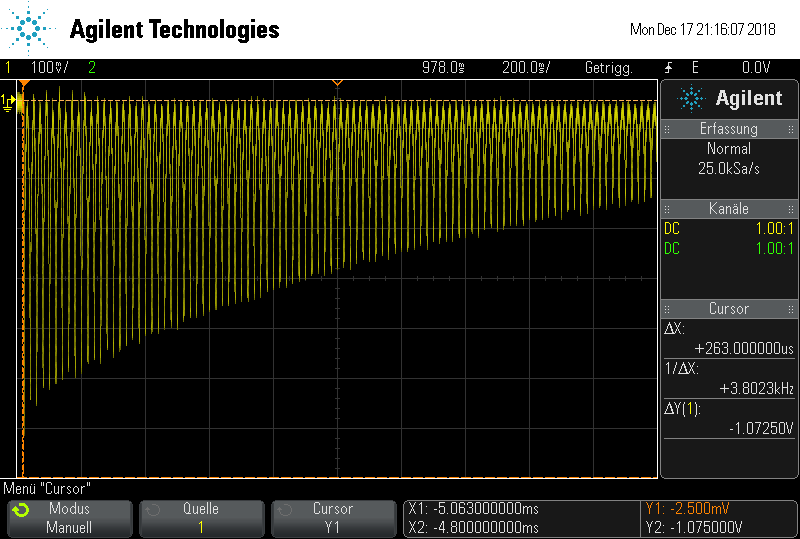
\includegraphics[width=0.8\textwidth]{rohdaten/mg_2.png}
  \caption{Aufnahme der Meiboom-Gill-Methode mit eingestelltem Pulsabstand.}
  \label{fig:MG}
\end{figure}
\input{build/MG.tex}
Um die transversale Relaxationszeit $T_2$ zu berechnen werden die Minima mit der
Funktion \texttt{find\_peaks} des Pythonpakets \texttt{scipy.signal} bestimmt und
sind in Tabelle \ref{tab:MG} aufgelistet.
Eine Regression ist mit einer Formel
der Form
\begin{align*}
  U(t) = U_0 \cdot \text{e}^{-\frac{t}{T_2}}
\end{align*}
mit $t = 2\tau$ durchgeführt worden. Die daraus erhaltenen Parameter sind
\begin{align*}
  U_0 &= -\SI{588(3)}{\milli\volt} \\
  T_2 &= \SI{1.657(17)}{\second}.
\end{align*}
Regression und ermittelte Extrema der induzierten Spannung in Abhängigkeit des
Zeitabstands der Pulse ist in Abbildung \ref{plt:MG} dargestellt.
\begin{figure}[htb]
  \centering
  \includegraphics{build/MG.pdf}
  \caption{Graphische Darstellung der Minima der $\SI{180}{\degree}$-Peaks.}
  \label{plt:MG}
\end{figure}
\FloatBarrier

\subsubsection{Carr-Purcell-Methode}
Für die Aufnahme der Cerr-Purcell-Methode wurden die Shim-Parameter auf die
folgenden Werte eingestellt:
\begin{align*}
  x &= -\num{0.84} \\
  y &= -\num{4.92} \\
  z &= +\num{3.72} \\
  z^2 &= +\num{2.84}
\end{align*}
Zudem wurde die Lamor-Frequenz auf $\omega_\text{L} = \SI{21.71223}{\mega\hertz}$
verwendet. Die aufgenommene Sequenz ist in Abbildung \ref{fig:CP} dargestellt.
Des Weiteren ist in Abbildung \ref{fig:CP2} die Pulssequenz für einen
deutlich größeres Zeitintervall dargestellt.
\begin{figure}[htb]
  \centering
  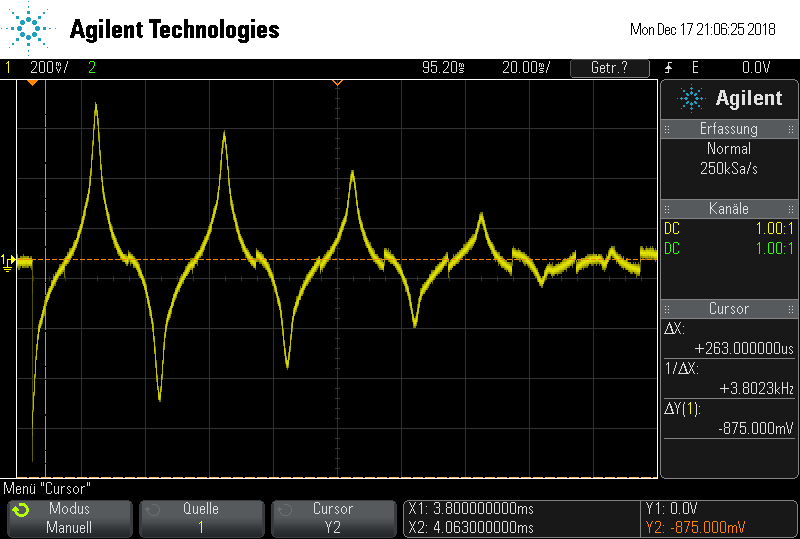
\includegraphics[width=0.8\textwidth]{rohdaten/cp_2.png}
  \caption{Am Oszilloskop aufgenommene Sequenz der Carr-Purcell-Methode.}
  \label{fig:CP}
\end{figure}
\begin{figure}[htb]
  \centering
  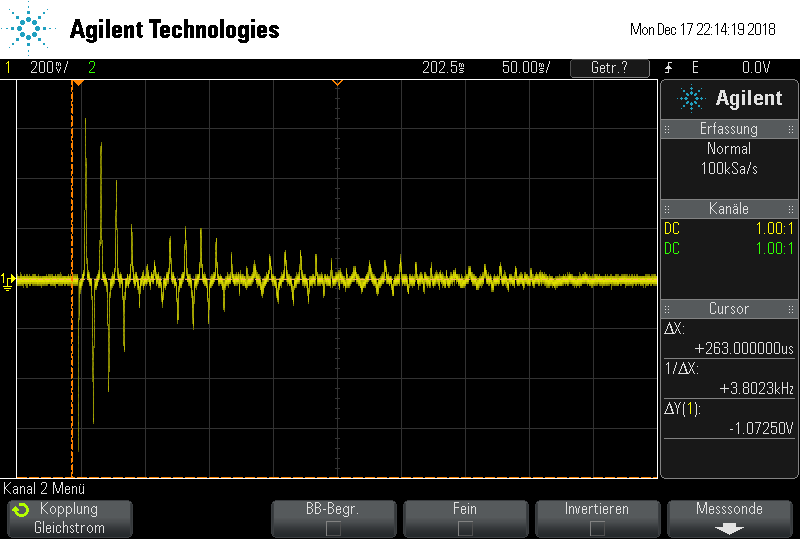
\includegraphics[width=0.8\textwidth]{rohdaten/cp_3.png}
  \caption{Am Oszilloskop aufgenommene Carr-Purcell-Methode für einen längeren Zeitraum.}
  \label{fig:CP2}
\end{figure}
Eine quantitative Auswertung des Pulshöhen in Abbildung \ref{fig:CP} wäre möglich,
jedoch nicht sinnvoll.
Wie im Theorieabschnitt \ref{sec:CP-und-MG} dargelegt tritt hier bei nicht
exakt eingestellter Länge des \SI{180}{\degree}-Pulses eine systematische
Abweichung auf, weil die Magnetisierung nicht exakt um \SI{180}{\degree}
gedreht wurde.
Aufgrund dessen ist die ermittelte Magnetisierung in der $\vec{x}'\vec{y}'$-Ebene
geringer, als sie eigentlich wäre.
Die Ungenauigkeit der Einstellung des \SI{180}{\degree}-Pulses ist klar in
Abbildung \ref{fig:CP2} zu erkennen.
Für einen größeren Zeitraum addieren sich die Zeitabweichungen des \SI{180}{\degree}-Pulses
zum perfekten Wert immer weiter auf, bis die Magnetisierung wieder in die
Ebene gedreht wird.
Dieser Effekt erzeugt die in der Abbildung erkennbare Oszillation der
Maxima der Pulssequenz.
\FloatBarrier


\subsection{Bestimmung der Halbwertsbreite}
Zur Bestimmung der Halbwertsbreite $t_{\sfrac{1}{2}}$ eines Spin-Echos wird das
Maximum des Spin Echos bestimmt. Bei halber Höhe des Maximums wird die Differenz
der entsprechenden $\tau$ Werte berechnet. Graphisch ist die durch die Messung
bestimmte Halbwertsbreite in Abbildung \ref{plt:t12} durch die rote gestrichelte
Linie gekennzeichnet.
Zur Referenz ist in \ref{fig:t12} das zugehörige Bild der Sequenz am Oszilloskop zu sehen.
Dabei beträgt der Wert für die Halbwertsbreite
\begin{align*}
  t_{\sfrac{1}{2}} = \SI{8.55e-5}{\second}
\end{align*}
\begin{figure}[htb]
  \centering
  \includegraphics{build/halbwertsbreite.pdf}
  \caption{Messung eines Spin-Echos und Bestimmung der Halbwertsbreite.}
  \label{plt:t12}
\end{figure}
\begin{figure}[htb]
  \centering
  \includegraphics[width=0.7\textwidth]{rohdaten/halbwertsbreite.png}
  \caption{Sequenzbild des Spin-Echos zur Bestimmung der Halbwertsbreite.}
  \label{fig:t12}
\end{figure}
\FloatBarrier

\subsection{Bestimmung der Diffusionskonstante}
Die Diffusionskonstante wurde mittels Spin-Echo-Verfahren bestimmt. Dabei wurde
ein maximaler Gradient des Magnetfeldes in $z$-Richtung eingestellt. Dieser beträgt
$z = -\num{9.00}$. Durch diese Anpassung wird ein möglichst inhomogenes Magnetfeld
erzeugt und somit ein Diffusionseffekt messbar.
Um die Diffusionskonstante $D$ berechnen zu können, muss zunächst der Faktor
$G$ berechnet werden. Dazu wird $G$ mittels der Formel
\begin{align*}
  G = \frac{4\cdot 2.2}{d \gamma t_\frac{1}{2}}
\end{align*}
mit $d = \SI{4.4}{\milli\meter}$ zu
\begin{align*}
  G = \SI{0.0874}{\tesla\per\meter}
\end{align*}
berechnet.
Dazu wird der erste Echo-Puls bei $t = 2\tau$ für verschiedene Pulslängen
verwendet. Die Regression wird mit Hilfe
einer Funktion der Form von Gleichung \eqref{eqn:DiffusionsBestimmung} durchgeführt. Verwendet wurden die
Messdaten aus Tabelle \ref{tab:dif}.
\input{build/diff.tex}
Grapisch dargestellt ist in Abbildung
\ref{plt:diff} das erste Echo in Abhängigkeit der Pulsabstände und die Regression
zur Bestimmung der Diffusionskonstante.
\begin{figure}[htb]
  \centering
  \includegraphics{build/diffussion.pdf}
  \caption{Erstes Echo $U$ in Abhängigkeit vom Pulsabstand $\tau$ und Regression
  zur Bestimmung der Diffusionskonstanten $D$.}
  \label{plt:diff}
\end{figure}
Als Fitparameter ergeben sich:
\begin{align*}
  U_0 &= \SI{628(6)}{\milli\volt} \\
  D &= \SI{1.74(5)e-9}{\square\meter\per\second}
\end{align*}

\subsection{Bestimmung der Viskosität}
Die Viskosität wird durch die Funktion
\begin{align*}
  \eta(T) = \rho \alpha \left(t - \delta\right)
\end{align*}
\input{build/viskos.tex}
berechnet. Es wurden die Werte $\rho = \SI{1000}{\kilo\gram\per\cubic\meter}$
und $\alpha = \SI{1.2024d-9}{\square\meter\per\square\second}$ verwendet. Mit
Hilfe der gegebenen Werte aus Tabelle \ref{tab:viskos} ist durch eine lineare
Regression ein Wert von
\begin{align*}
  \delta = \SI{0.48}{\second}
\end{align*}
berechnet worden. Wird dieser Wert mit dem gemessenen Zeitintervall
$t = \SI{930}{\second}$ in die Formel für die Viskosität eingesetzt,
so ergibt sich ein Wert von
\begin{align*}
  \eta = \SI{9.4d-4}{\kilo\gram\per\meter\per\second}.
\end{align*}

\subsection{Bestimmung des Molekülradius}
\label{sec:AuswMolekuel}
Der Molekülradius $r$ wird durch die Stockesschen Formel
\begin{align*}
  r = \frac{k_\text{B} T}{6\pi\eta D}
\end{align*}
mit der Boltzmann-Konstante $k_\text{B}$, der Viskosität bei Raumtemperatur $T = \SI{25}{\degree}$
und der zuvor berechneten Diffusionskonstante $D$. Daraus ergibt sich ein Wert von
\begin{align*}
  r = \SI{1.33}{\angstrom}
\end{align*}
Um diesen Wert einordnen zu können, wird zum Vergleich ein Referenzwert berechnet.
Dazu wird zum einen die Annahmen verwendet, dass die Moleküle in einer
hexagonal dichten Kugelpackung (hcp) befinden. Dabei beträgt die Raumfüllung
$\SI{74}{\percent}$. Mit der daraus resultierenden Molekülmasse von Wasser
$m_{H_2O} = \SI{28.89d-27}{\kilo\gram}$ und der Dichte von
$\rho = \SI{997.04}{\kilo\gram\per\cubic\meter}$ \cite{hcp} ergibt sich der
Molekülradius
\begin{align*}
  r_\text{hcp} = \left(\frac{m_{H_2O}\cdot 0,74}{\frac{4}{3} \pi \rho }\right)^\frac{1}{3} = \SI{1.71}{\angstrom}.
\end{align*}
Als zweite Annahme wird ein van-der-Waals Gas am kritischen Punkt angenommen,
daraus ergibt sich
\begin{align*}
  r_\text{VdW} = \left(\frac{3kT_\text{k}}{128\pi P_\text{k}}\right)^\frac{1}{3} = \SI{1.44}{\angstrom}.
\end{align*}
Dabei ist $T_\text{k} = \SI{647.05}{\kelvin}$ und $P_\text{k} = \SI{22.04e6}{\pascal}$ \cite{VdW}.


%Carr-Purcell diskutieren, warum quantitativ nicht auswertbar
%Oszillationen bei höheren Zeiten: Winkeldelta addiert sich iwann
%wieder auf 180°, damit wieder Signal
%T1-Messung
%Anstelle des Fits in der Anleitung (bei dem M0 quasi zufällig gewählt werden muss):
%Nichtlinearer Fit an logarithmierte Messwerte
%Fit der Form M0 * (1 - 2*exp(-t/tau)) + M1
%mit Offset M1
%Bitte Form noch einmal genauer überprüfen

% \subsection{Unterkapiel}
% \label{sec:Unterkapitel}

% \begin{figure}
%   \centering
%   \includegraphics[width=\textwidth]{Plot.pdf}
%   \caption{Bildunterschrift}
%   \label{fig:Plot1}
% \end{figure}
